\chapter{The Software Project Architecture}\label{chap:arch}

In this chapter, we outline the conceptual design of the software package.
We describe individual parts and how they interact.
We talk about commands to execute the project.
\todoA{finish this when the chapter is really ready}


The software package was designed and developed with extensibility in mind.
It allows easily adding new features, specifying different subsets of data and converting them into various format without breaking older experiments.
Various libraries are utilized for both higher performance and easier maintainability.
Abstract classes are utilized for defining clear API and allow easy addition of new algorithms.

A special configuration file is utilized allowing to change the behaviour without touching the code base.
All classes and files have documentation strings which should be sufficient for detailed understanding.
In this chapter, we only describe the high-level overview.

A conceptual overview is outlined in \autoref{fig:conceptual_design}.
The flow of the programme is top to bottom.
Ellipses represent processes, rectangles data and cut rectangles input data.
The output is represented by \textit{result}.

First, unused reviews are dropped resulting in \textit{filtered reviews}.
Filtered reviews are added the information about the businesses they belong to in \texttt{join}.
The result is stored in the \textit{instance file}.

In addition to the provided data, external text analysis is used.
Entities and sentiment are extracted from all reviews and
subsequently not used reviews are dropped resulting in \textit{filtered entities and sentiment}.

The two files \textit{instance file} and \textit{filtered entities and sentiment} 
are used for generating instances with all necessary data represented by \textit{full instances}.
Full instances are split into pairs of training and testing sets for k-fold cross validation.

Next, \textit{experiments file} is loaded.
Information about classifier configuration is used to generate samples from \textit{train and test sets pairs}.
The samples have exactly the needed features for the particular classifier and necessary preprocessing is done
resulting in \textit{preprocessed instances}.

Preprocessed instances are used for training a model which is used for predicting test set.
The predictions are used for evaluation performance.
Evaluation results are saved into output files as defined in \textit{graphs specification} extracted from
the \textit{experiments file}.


\begin{figure}[h!!]
    \centering
	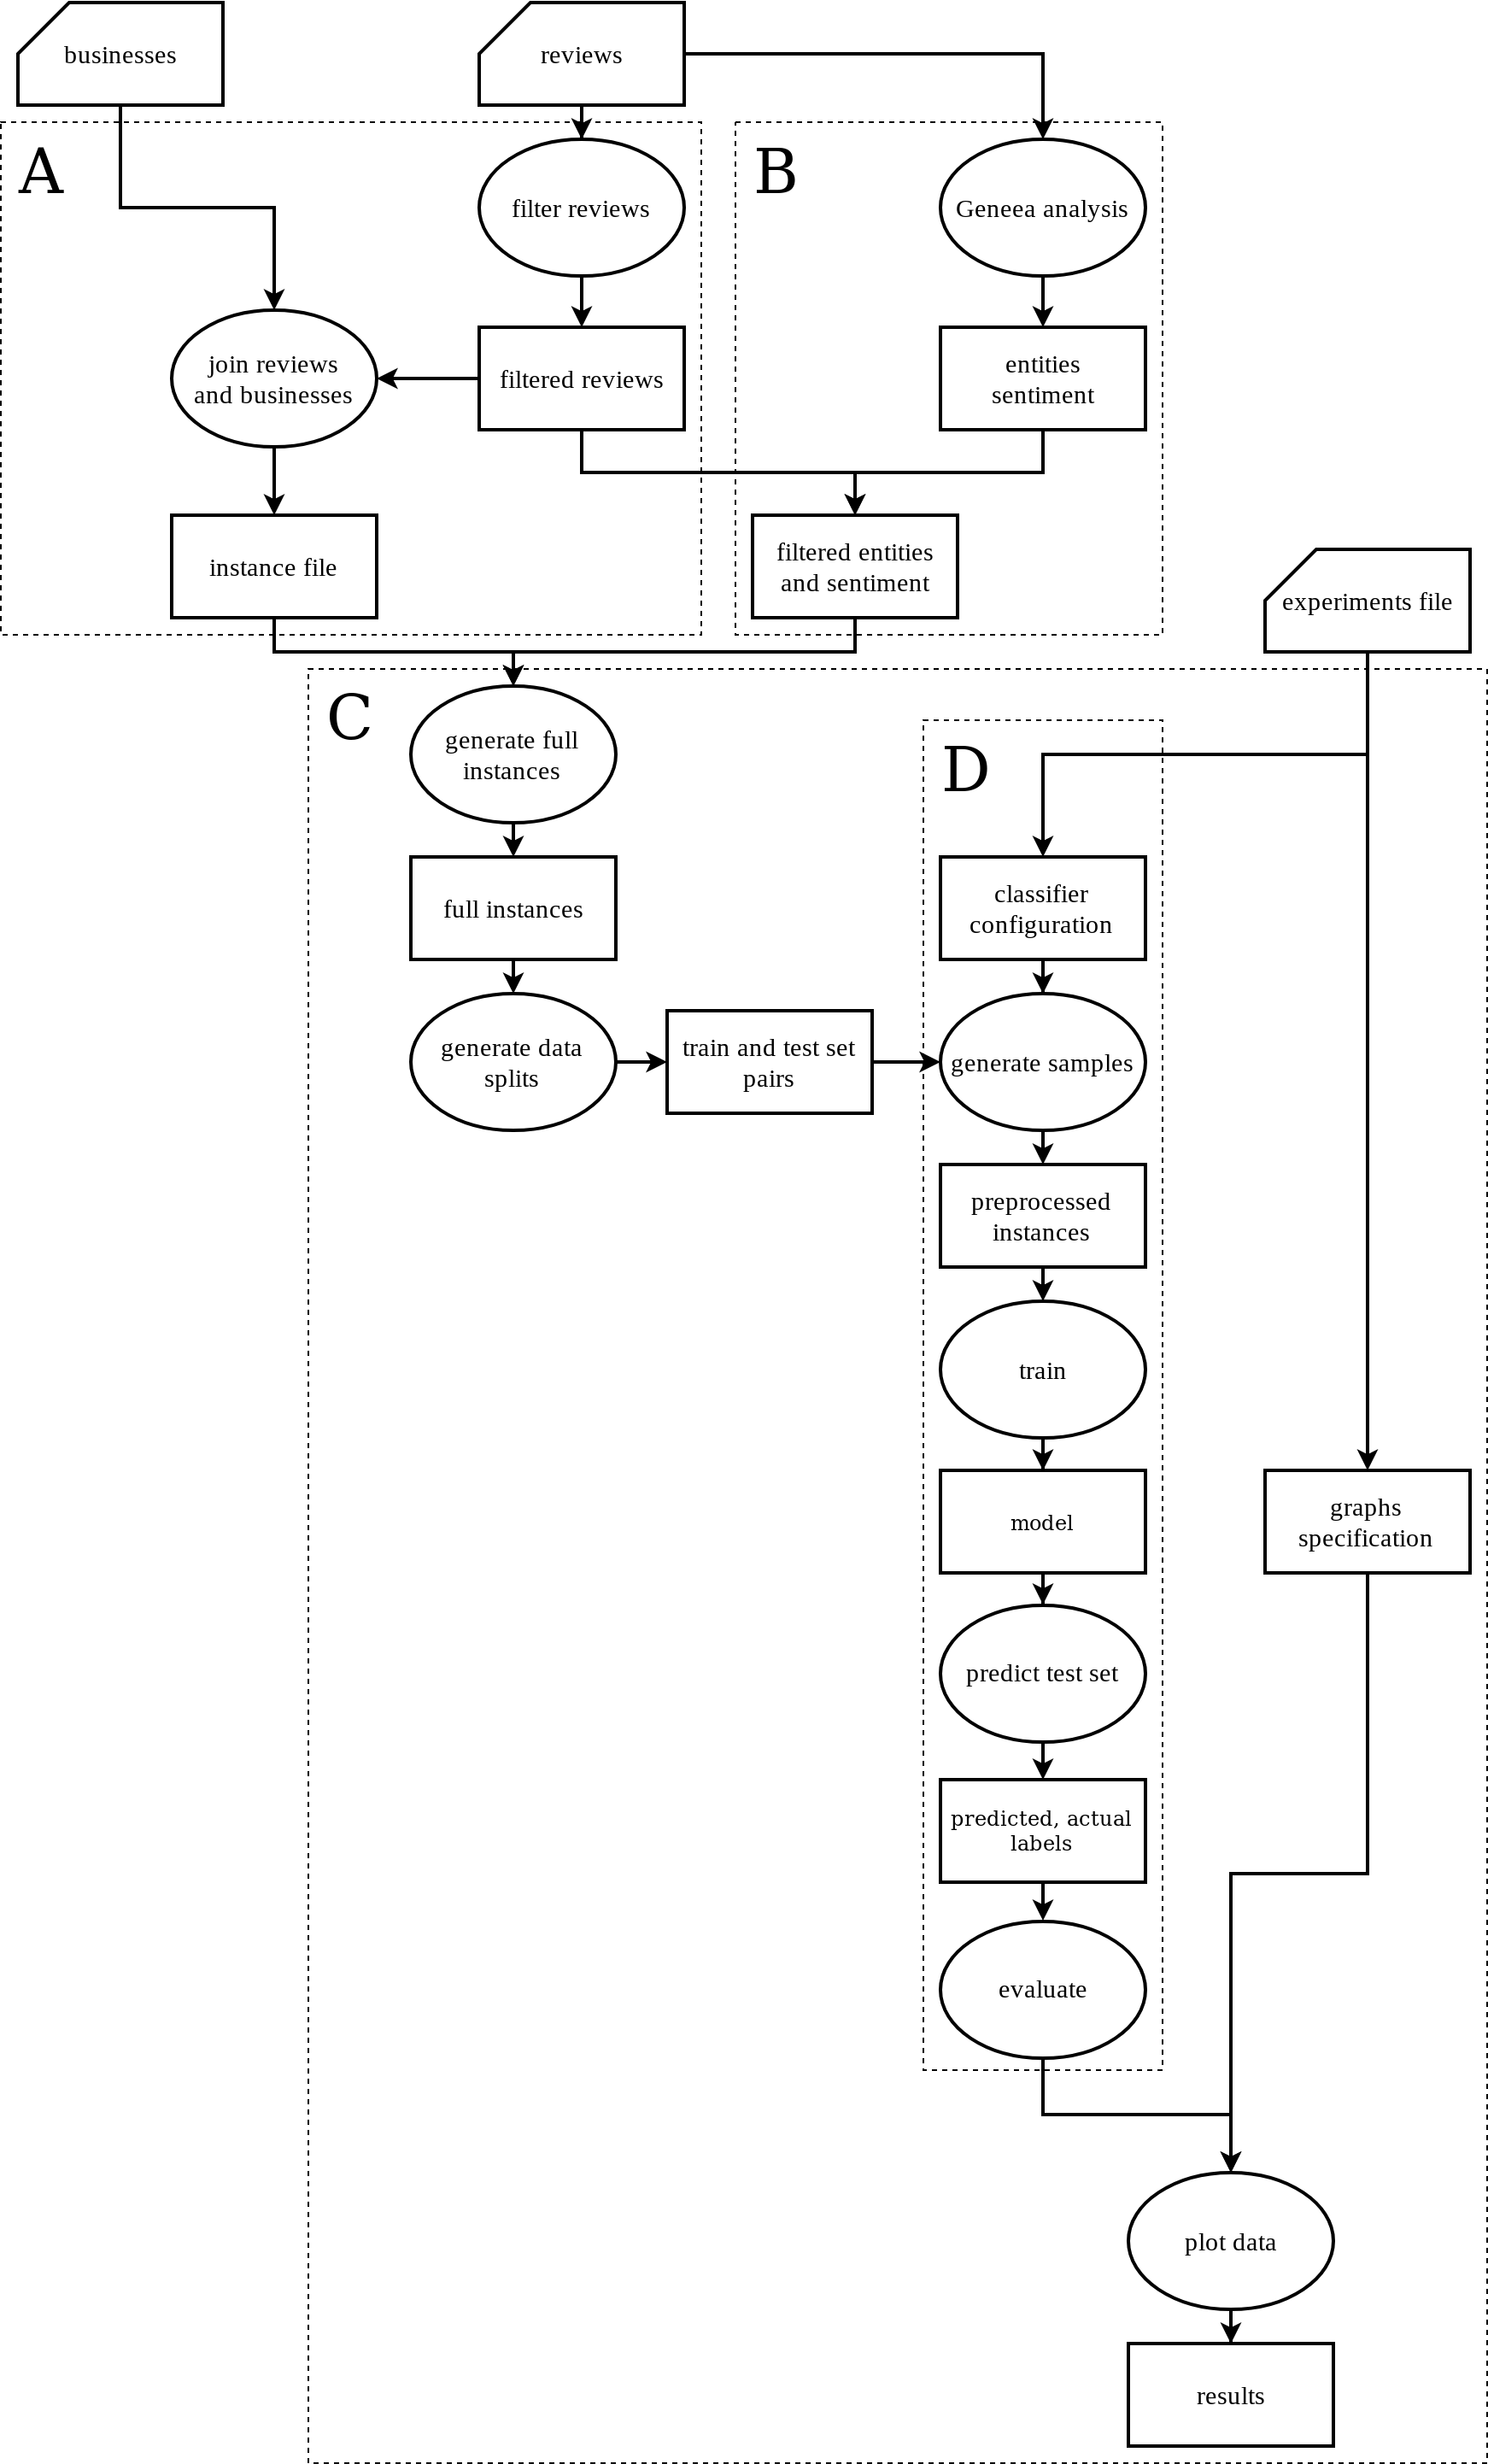
\includegraphics[width=\textwidth]{figures/conceptual_design.png}
	\caption{Conceptual Design}\label{fig:conceptual_design}
\end{figure}






\section{Parts Overview}

The project is implemented in three separate parts as shown in \autoref{fig:arch_process}.
\texttt{Prepare data} creates the instances file and corresponds to rectangle A in \autoref{fig:conceptual_design}.
\texttt{Add Geneea analysis} corresponds to rectangle B --- it creates filtered entities and sentiment.
The last part \texttt{Run experiments} does the entire training, evaluating and creating statistics process.
It is represented by rectangle C.
Subset of the last part is devoted to running the experiments; \texttt{run experiments} corresponds to rectangle D.

We describe each part in a separate subsection.

\begin{figure}[h]
    \centering
	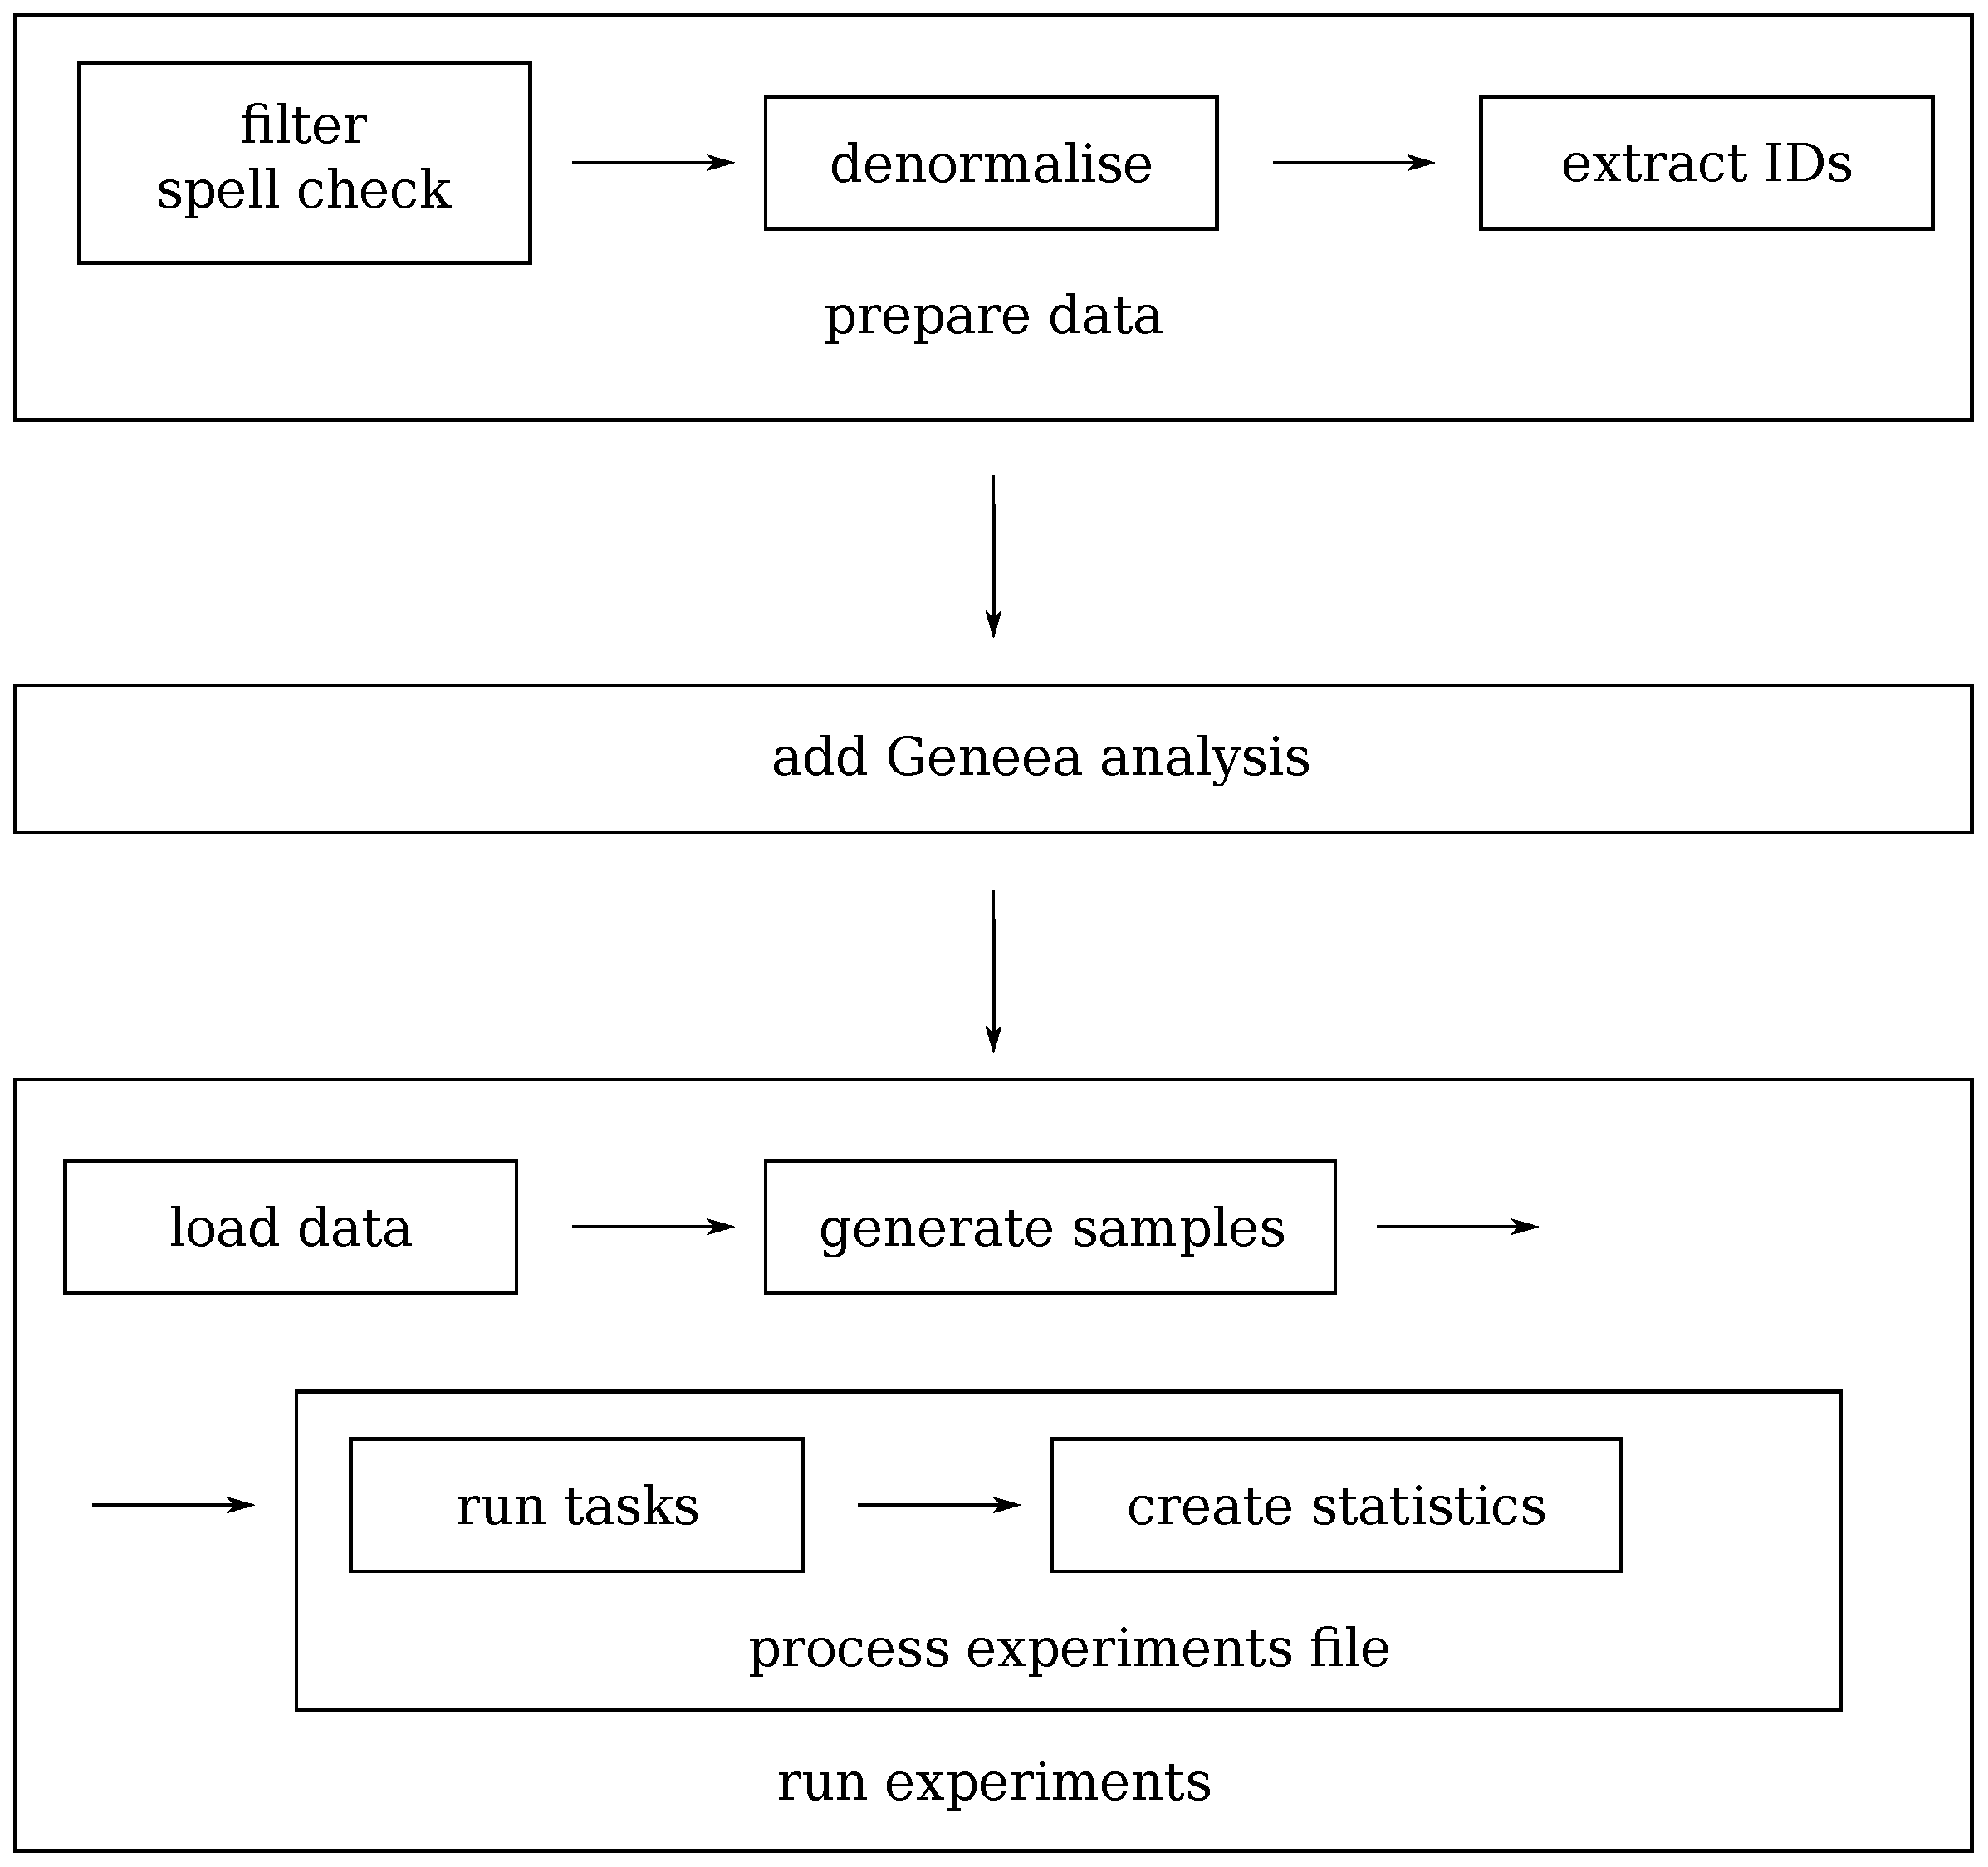
\includegraphics[width=10cm]{figures/arch_process.eps}
	\caption{Architecture Design}\label{fig:arch_process}
\end{figure}


\subsection{Data Preparation} 

All scripts for preparing data are in the folder \texttt{denormalization}.
These scripts take the dataset and produce an instance file.
Filtering of reviews as specified in \autoref{app:prepr} is done.
Because reviews are processed through the spellchecker for filtering,
the output is added into data as a byproduct.
In \texttt{denormalize}, businesses are joined.

At the end, in addition to the instance file, ID file is also created.
It contains extracted IDs from the instance file.
This is used to tell the Geneea analyzer what reviews are needed to save bandwidth,
because the Geneea analysis is performed on a remote server.

\subsection{Geneea Analysis}

Geneea analysis uses external tools for extracting more linguistics features.
Thorough description can be found in \autoref{app:geneea}.
The analysis extracts entities and sentiment from all reviews.
Subsequently, it takes filtered reviews in the form of ID file to drop all unnecessary data.
The result is stored in a file, which has to be transferred to the local computer in order to be able to continue with the next part.





\subsection{Run Experiments}

This entire part is handled by \texttt{process\_data.py}, which executes other parts of the code.
Loading data and generating samples is handled by \texttt{load\_data.py}.
Preprocessing is defined in directory \texttt{preprocessors} and classification models in \texttt{classifiers}.
Finally, creating statistics is handled by \texttt{my\_statistics.py}.


\subsubsection{Load Data}

The \textit{instance} and \textit{filtered entities and sentiment} files are loaded and
converted into full instances in memory.
This is handled by class \texttt{Data}.
Subsequently, splits are generated and stored in an instance of \texttt{Sample}.
Splits are still raw data, features are generated in the next step.

\subsubsection{Generate Samples}

When \texttt{process\_data.py} loads classifier configuration,
it uses the loaded instances to generate features for the train and test sets.

\subsubsection{Run Experiments}

Running experiments is implemented as a pipeline being fed with the generated sets and outputting predicted labels.
The units of the pipeline are preprocessors and a classifier.
Preprocessors are implemented as children of \texttt{preprocessors/preprocessingbase.py} and classifiers
as \texttt{classifiers/classifierbase.py}.
The pipeline is first fed with training data to built a model.
Subsequently, testing data is passed and predicted labels are stored.

The predicted labels are compared to the actual labels and several evaluation metrics are calculated.
Those are stored in an instance of \texttt{DataGraph}, which serves as a buffer until all results are gathered.

\subsubsection{Create Statistics}

When all experiments are run, graph specification is read.
Data from \texttt{DataGraph} is used to plot graphs as per the specification.
An instance of this class is passed to \texttt{Statistics},
which handles the actual data plotting and writing to files.
